\chapter{Mapping Techniques for SDOG and the Extension Method} \label{chap:mapping}
The previous two chapters discussed methods for creating hierarchical grid geometry to be used in a 3D DGGS.
However, grid geometry on its own is not sufficient for functioning as a DGGS.
Geospatial data, which represents locations in physical space, need to be mapped to the domain of the grid system and vice versa.
In a 2D DGGS, this is handled by the projection method and its inverse.
A projection $P$ maps the surface of a sphere (physical domain) to the grid domain; the inverse $P^{-1}$ does the opposite.
A 3D DGGS requires a similar operation but instead maps the volume of a ball (physical domain) to some other volume (grid domain).
We refer to these mapping functions by $M$ to distinguish them from their 2D projection counterparts.


Since our modifications of SDOG have the same grid domain as the physical space, such mappings are not strictly required; despite this, they can still be useful.
As we will explore in Chapter~\ref{chap:coding}, the regularity of midpoint refinement in SDOG allows for efficient encoding and decoding algorithms, which is not the case for our modifications.
A mapping between conventional SDOG and the modified grids allows for efficient encoding and decoding with inputs and outputs converted between the two representations.


On the other hand, for 3D DGGS's resulting from the extension of a polyhedron-based 2D DGGS, it is clear such mappings \textit{are} needed.
Beyond their necessity, though, these mappings also allow for other properties of the grid system to be achieved. Most notably, volume preservation can be improved with appropriate mapping functions.


In this chapter, we present two sets of mapping functions for use with our SDOG modifications and our grid extension method:
the first is a set of radial mappings used for both approaches;
the second is a set of latitude mappings for SDOG, which operate on similar principles as the radial ones.
We do not provide mappings for the surface coordinates in the grid extension method, as this is handled by the projection method of the input DGGS.
We present the inverse mappings first, as the geometric intuition for the role of these operations is more apparent than the forward.
For SDOG, the inverse takes conventional SDOG and maps it to the modified grids presented in Chapter~\ref{chap:sdog}
For grid extension, the inverse takes the prismatoid grid and maps it to the corresponding grid in physical space.
We then derive the forward mappings from the inverses. 


\section{Radial Mappings} \label{chap:6:radial}
Goal is to define function $M_r(r)$. Consider radius to be normalized with $\hat{r} = r / R_\mathrm{max}$.


We first note the similarity between SDOG and the grid extension method as they both use semiregular degenerate refinement.
Referring back to Figure~\ref{fig:sdog-shells} for SDOG and comparing it to Figure~\ref{fig:prismatoid-shells} for the extension method, radial splits have the same effect and structure.
Therefore, Equation~\ref{eq:shellVolume} also is true for the grid extension method.
However, the refinement factor for the extension method is not always 1:8, as it depends on the surface refinement factor, and therefor the best placement for the split then is not necessarily $\alpha = 1/2$.
Instead, we want $\alpha^3 = 1 / f^{\ 3}$ and thus $\alpha = 1/f$.
Therefore, SDOG mappings are special case of extension one where $f = 2$.

\begin{figure}[ht!]
	\centering
	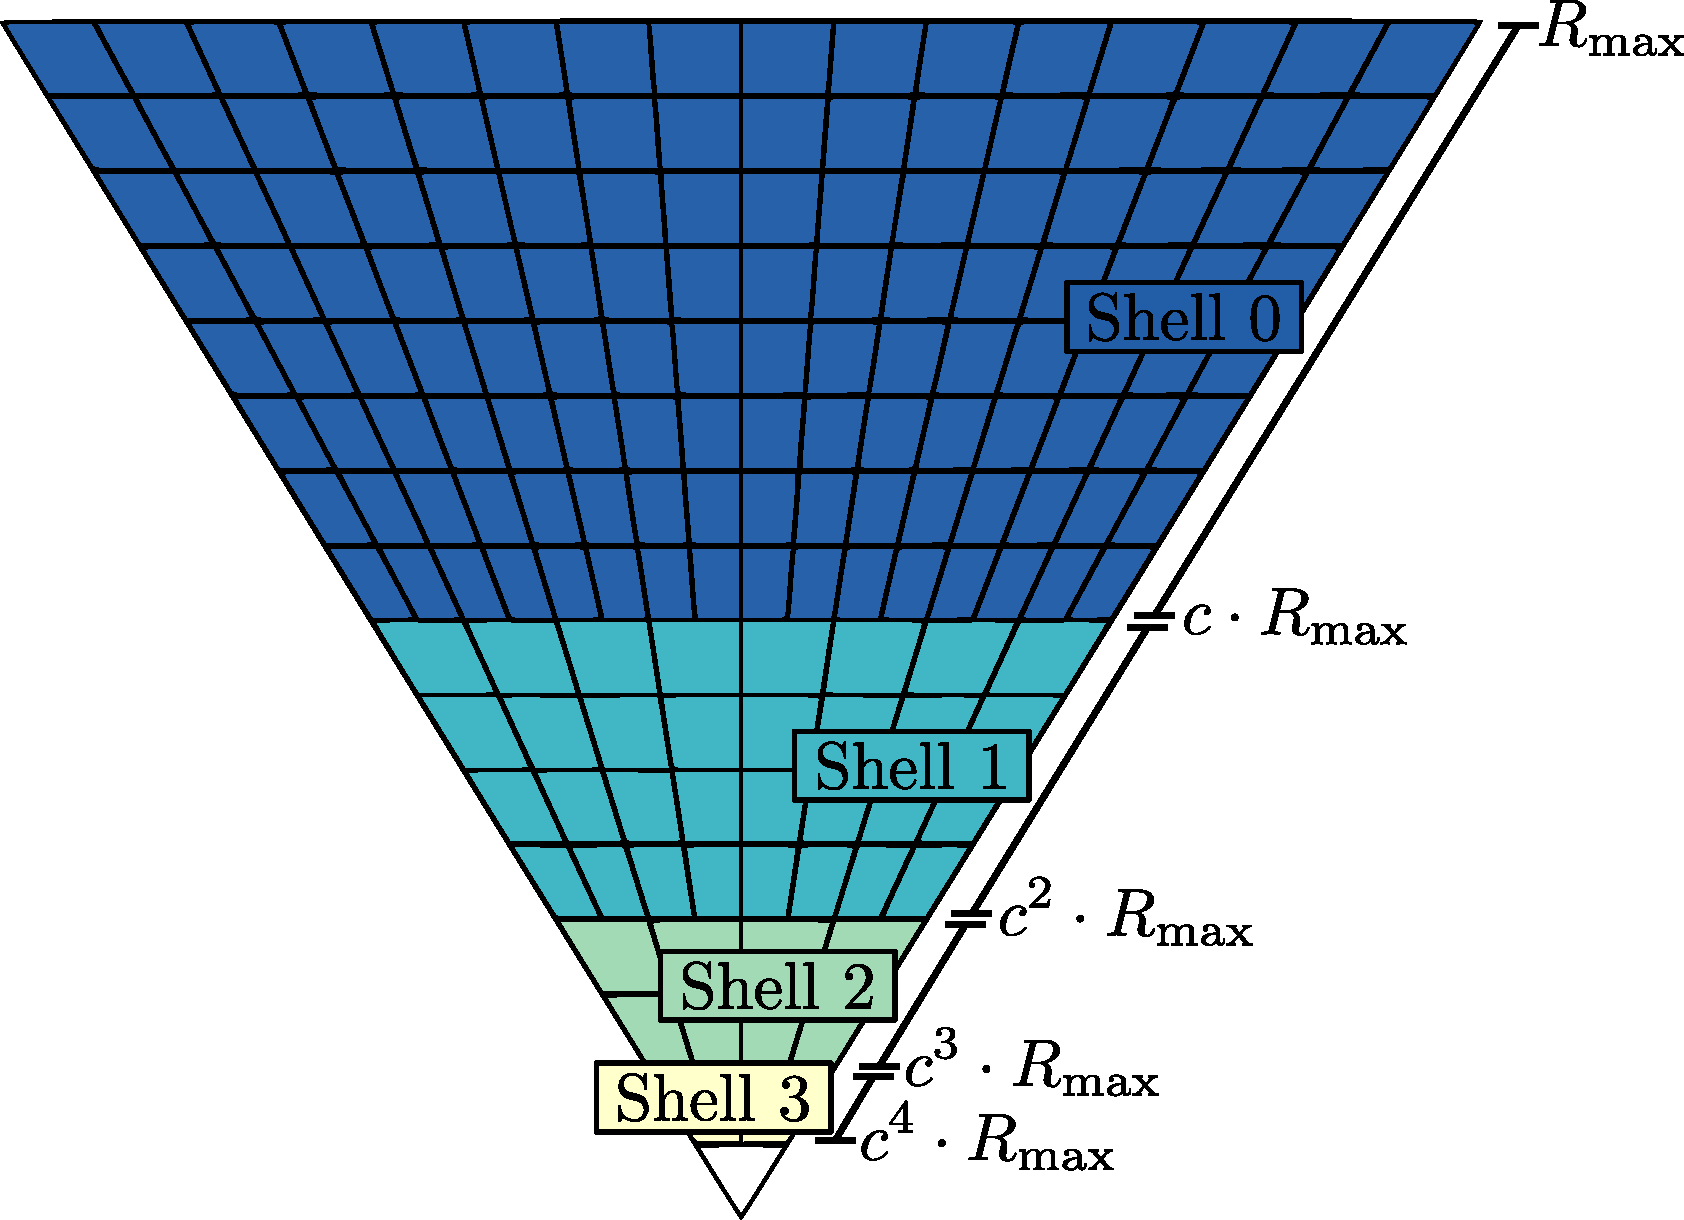
\includegraphics[width=0.675\textwidth]{prismatoid-shells.pdf}
	\caption[Spherical shells that result from the grid extension method]{
		Radial splits of central layers divide the grid into regions that represent spherical shells.
		At $k$ levels of refinement there are $k$ shells and the central layer.
		These shells are similar and should have a mapped volume proportional to the number of cells they contain
	}
	\label{fig:prismatoid-shells}
\end{figure}

Radii at powers of $1/2$ in the grid should be mapped to corresponding powers of $\alpha$ in physical domain.
For a given $\hat{r}$ then, need to find one above and one below.
Shell $s = \lfloor \log_{0.5} \hat{r} \rfloor$.
Can then find these splits in both grid and physical domain by raising to appropriate power.
%
\begin{equation*}
\ell_p = \alpha^{s+1}, \quad u_p = \alpha^s, \quad \ell_g = 0.5^{s + 1}, \quad \text{and} \quad u_g = 0.5^s.
\end{equation*}
%
Mapping can be achieved then by finding a percent between $\ell_g$ and $u_g$ and then mapping said percent between $\ell_p$ and $u_p$.
Call percent $d$, then
%
\begin{equation} \label{eq:radialInvD}
d = \frac{ \hat{r} - \ell_g }{ u_g - \ell_g }
\end{equation}
%
How $d$ is interpolated between $\ell_p$ and $u_p$ affects volume preservation.
Using a linear interpolation is the same as conventional SDOG and latitude method, cubic is the volume method, and a power of $t$ gives the balanced method.
Thus, the general formulation is
%
\begin{equation} \label{eq:radialInv}
M_r^{-1}(\hat{r}) = \sqrt[t]{ d u_p^{t} + \left( 1 - d \right) \ell_p^{t} }
\end{equation}
%
which is just a more general form of Equation~radialblend.


From this we can derive the forward mapping by inverting the inverse.
Can solve Equation~\ref{eq:radialInv} for $d$ to get
%
\begin{equation} \label{radialForwD}
d = \frac{ \hat{r}^{\,t} - \ell_p^{\,t} }{ u_p^{\,t} - \ell_p^{\,t} }
\end{equation}
%
and solve Equation~\ref{eq:radialInvD} for $\hat{r}$ to get
%
\begin{equation} \label{eq:radialForw}
M_r (\hat{r}) = d u_p + \left( 1 - d \right) \ell_p 
\end{equation}
%
Uppers and lowers are the calculated the same, but the shell is now $s = \lfloor \log_{c} \hat{r} \rfloor$.


The results of this mapping for different values of $t$ applied to the grid extension method are shown in Figure~X. These mappings have the side effect of changing the aspect ratio of cells in grid space as compared to in physical space. This means that when determining the refinement parameters needed to achieve the desired aspect ratio, the cells in physical space should be considered as opposed to grid space.
This is accomplished by setting the value of $\nu$ in Equations~X and X to be $(1 - \alpha)$.

\section{Latitude Mappings for SDOG} \label{chap:6:latitude}

%\section{Mapping Modified SDOG Grids} \label{sec:mapping}
By modifying the splitting surfaces used for subdivision, any SDOG indexing operations that depend on the location of cells in the grid will no longer function properly.
Examples of these operations include point to cell queries, which give the cell that contains a given point, and index inversion, which calculates the location and geometry of a cell from its index.
The obvious solution is to simply redefine these operations on the new geometry, however, this is not necessarily practical as it would have to be done individually for each modified grid.
Additionally, the more complex geometry of the modified grids may make these algorithms more difficult to design and/or more computationally expensive to perform as compared to the ones for conventional SDOG.
A better solution is to find a mapping (and corresponding inverse mapping) between a conventional SDOG grid and the grid resulting from the modified subdivision scheme.
Given this mapping, all indexing operations can be done using the standard algorithms, with inputs and outputs converted between the conventional SDOG grid and the modified one accordingly.


For the stationary subdivision schemes this mapping is straightforward.
Since only the latitudinal splitting surface of SG cells is modified, latitudes in the range $[0, \pm\frac{\pi}{4})$ should be mapped to the range $[0, \pm\alpha_{\phi}^{SG} \frac{\pi}{2})$ and likewise the range $[\pm\frac{\pi}{4}, \pm\frac{\pi}{2}]$ to the range $[\pm\alpha_{\phi}^{SG} \frac{\pi}{2}, \pm\frac{\pi}{2}]$.
This can be done with a simple linear map, and the inverse follows trivially.


For the non-stationary schemes this mapping is more complicated.
We wish to define a function $M \colon (\phi, r) \rightarrow (\phi, r)$ that converts a latitude and radius in a conventional SDOG grid to the corresponding latitude and radius in the modified grid (longitude does not need to be mapped, as it is not changed between the two grids).
The two coordinates act independently of each other, so we can split this function into its two components, $M_{\phi}(\phi)$ and $M_{r}(r)$, and derive each one and its inverse individually.
This is done by parameterizing points inside an NG cell using the function(s) used to calculate its splitting surfaces (Eq.~(\ref{eq:convex}) for conventional SDOG and Eq.~(\ref{eq:radVol}) and (\ref{eq:latVol}) for the modified grid).
NG cells are used for this purpose as all children cells are also NG, and therefore use the same formulations for calculating splitting surfaces.
By finding the boundaries of the coarsest NG cell that contains a given point, these parameterizations can be used to go from one space to the other by finding a relationship between them---in this case $d = \alpha = p$---all of which can be done in constant time.
The final formulations are as follows, with the full derivation found in Appendix \ref{app:map}.
Let $R_m$ be the radius of the grid.
Latitude forward:
%
\begin{equation*}
M_{\phi}(\phi) = \sin^{-1} \left( d u_{v} + \left( 1 - d \right) \ell_{v} \right), \quad \text{where}
\end{equation*}
%
\begin{equation*}
d = \frac{\frac{2\phi}{\pi} - \ell_{c}}{u_{c} - \ell_{c}},
\end{equation*}
%
\begin{equation*}
u_{c} = 1 - \left( \frac{1}{2} \right)^{ \left\lceil \log_{0.5} \left( 1 - \frac{2\phi}{\pi} \right) \right\rceil }, \quad u_{v} = 2 u_{c} - u_{c}^{2}.
\end{equation*}
%
\begin{equation*}
\ell_{c} = 1 - \left( \frac{1}{2} \right)^{ \left\lfloor \log_{0.5} \left( 1 - \frac{2\phi}{\pi} \right) \right\rfloor }, \quad \text{and} \quad \ell_{v} = 2 \ell_{c} - \ell_{c}^{2}.
\end{equation*}
%
%
Radius forward:
%
\begin{equation*}
M_{r}(r) = R_{m} \sqrt[3]{ d u^{3} + \left( 1 - d \right) \ell^{3} }, \quad \text{where}
\end{equation*}
%
\begin{equation*}
d = \frac{\frac{r}{R_{m}} - \ell}{u - \ell},
\end{equation*}
%
\begin{equation*}
u = \left( \frac{1}{2} \right)^{ \left\lfloor \log_{0.5} \left( \frac{r}{R_{m}} \right) \right\rfloor }, \quad \text{and} \quad
\end{equation*}
%
\begin{equation*}
\ell = \left( \frac{1}{2} \right)^{ \left\lceil \log_{0.5} \left( \frac{r}{R_{m}} \right) \right\rceil }.
\end{equation*}
%
%
Latitude inverse:
%
\begin{equation*}
M^{-1}_{\phi}(\phi) = \frac{\pi}{2} \left( d u_{c} + \left( 1 - d \right) \ell_{c} \right), \quad \text{where}
\end{equation*}
%
\begin{equation*}
d = \frac{\sin \phi - \ell_{v}}{u_{v} - \ell_{v}},
\end{equation*}
%
\begin{equation*}
u_{c} = 1 - \left( \frac{1}{2} \right)^{ \left\lceil \log_{0.5} \left( \sqrt{1 - \sin \phi} \right) \right\rceil },
\end{equation*}
%
\begin{equation*}
\ell_{c} = 1 - \left( \frac{1}{2} \right)^{ \left\lfloor \log_{0.5} \left( \sqrt{1 - \sin \phi} \right) \right\rfloor },
\end{equation*}
%
%
and both $u_{v}$ and $\ell_{v}$ follow the same as the forward.
Radius inverse:
%
\begin{equation*}
M^{-1}_{r}(r) = R_m \left( d u + \left( 1 - d \right) \ell \right), \quad \text{where}
\end{equation*}
%
\begin{equation*}
d = \frac{ \left( \frac{r}{R_{m}} \right)^{3} - \ell^{3}}{u^{3} - \ell^{3}}
\end{equation*}
%
and both $u$ and $\ell$ follow the same as the forward.


In the case where a division by zero occurs, (i.e. when $u = \ell$ or $u_{c} = \ell_{c}$), the result of said division is treated as zero.
The latitude mappings assume $\phi \ge 0$, however, from symmetry a negative value of $\phi$ can easily be accommodated by using the absolute value and negating the final result.
This mapping is applicable to the first non-stationary scheme discussed in Section \ref{sec:method-nonStationary}; schemes derived from Eq.~(\ref{eq:beta}) cannot be mapped, as this formulation cannot easily be expressed in terms of a parameter.
In the future, other blending methods may be explored that allow for a similar mapping to be derived.




\section{Summary}